\chapter{Bezpieczeństwo aplikacji}

Do przechowywania wrażliwych danych użytkownika, takich jak hasło wykorzystywane są mechanizmy oferowane przez usługodawcę \textit{Auth0}. Dane przechowywane w bazie tego serwisu nie mają postaci zwykłego tekstu, a przechowywane za pomocą skrótu \textit{BCrypt}.

\textit{BCrypt} jest funkcją skrótu kryptograficznego, która została stworzona w celu przechowywania haseł statycznych, czyli haseł znanych wyłącznie osobie, która chce się uwierzytelnać, a nie dowolnych danych binarnych. \textit{BCrypt} wymaga stosowania soli, co wyróżnia ją od innych funkcji skrótu. Sól w algorytmie \textit{BCrypt} jest złożona z nastepujących elementów:

\begin{itemize}
	\item \textit{version} oznaczające wersję algorytmu \textit{BCrypt},
	\item \textit{rounds} jest to liczba z przedziału 04-99, która określa tzw. \textit{work factor} algorytmu, domyślna wartość tego pola to \$12,
	\item \textit{saltaddon} -- są to losowe 22 znaki, które mają za zadanie powiększać sól weryfikacja tego ciągu przebiega przy użyciu wyrażenia regularnego [./A-Za-z0-9] -- znaki te mogą być wylosowane przez użytkownika, bądź przez specjalnie zaprojektowany do tego celu algorytm. 
\end{itemize}

W \textit{Auth0} zarówno dane \textit{REST-owe}, jak i przekazywane w ruchu sieciowym są szyfrowane. Cała komunikacja sieciowa wykorzystuje protokół TLS (\textit{Transport Layer Security}) w wersji 1.2 (będący rozwinięciem protokołu SSL), z co najmniej 128-bitowym szyfrowaniem AES (\textit{Advanced Encryption Standard}). Do wymiany kluczy wykorzystywany jest mechanizm \textit{ECDHE\_RSA} oparty na protokole \textit{Diffiego-Hellmana} z podpisem generowanym przy użyciu kryptograficznego algorytmu asymetrycznego RSA (\textit{Rivest–Shamir–Adleman}). 

Usługi świadczone przez serwis \textit{Auth0} zaprojektowane są z myślą o wysokiej dostępności i odporności. Aplikacje korzystające z \textit{Auth0} są częściowo zabezpieczone przed atakami typu \textit{Odmowa usługi} czy \textit{Uwierzytelnianie}. Mają one wbudowane funkcje ograniczania szybkości i automatycznego blokowania. Ponadto konta użytkowników zabezpieczone są za pomocą domyślnie wbudowanego modułu weryfikacji autentyczności użytkownika przy użyciu adresu e-mail. Każdy użytkownik systemu otrzymuje unikalny JWT (\textit{JSON Web Token}), który pozwala na rozróżnianie i sprawdzanie autentyczności użytkowników aplikacji. Aplikacja została zabezpieczona przed skopiowaniem linku do panelu użytkownika zalogowanego i wklejeniu go do innego okna przeglądarki w celu uzyskania dostępu. W~ momencie takiej próby użytkownik zostaje poinformowany, że nie ma uprawnień do przeglądania treści danej strony (rys. \ref{Rys:no_access}). 

\newpage

\begin{figure}[h]
	\centering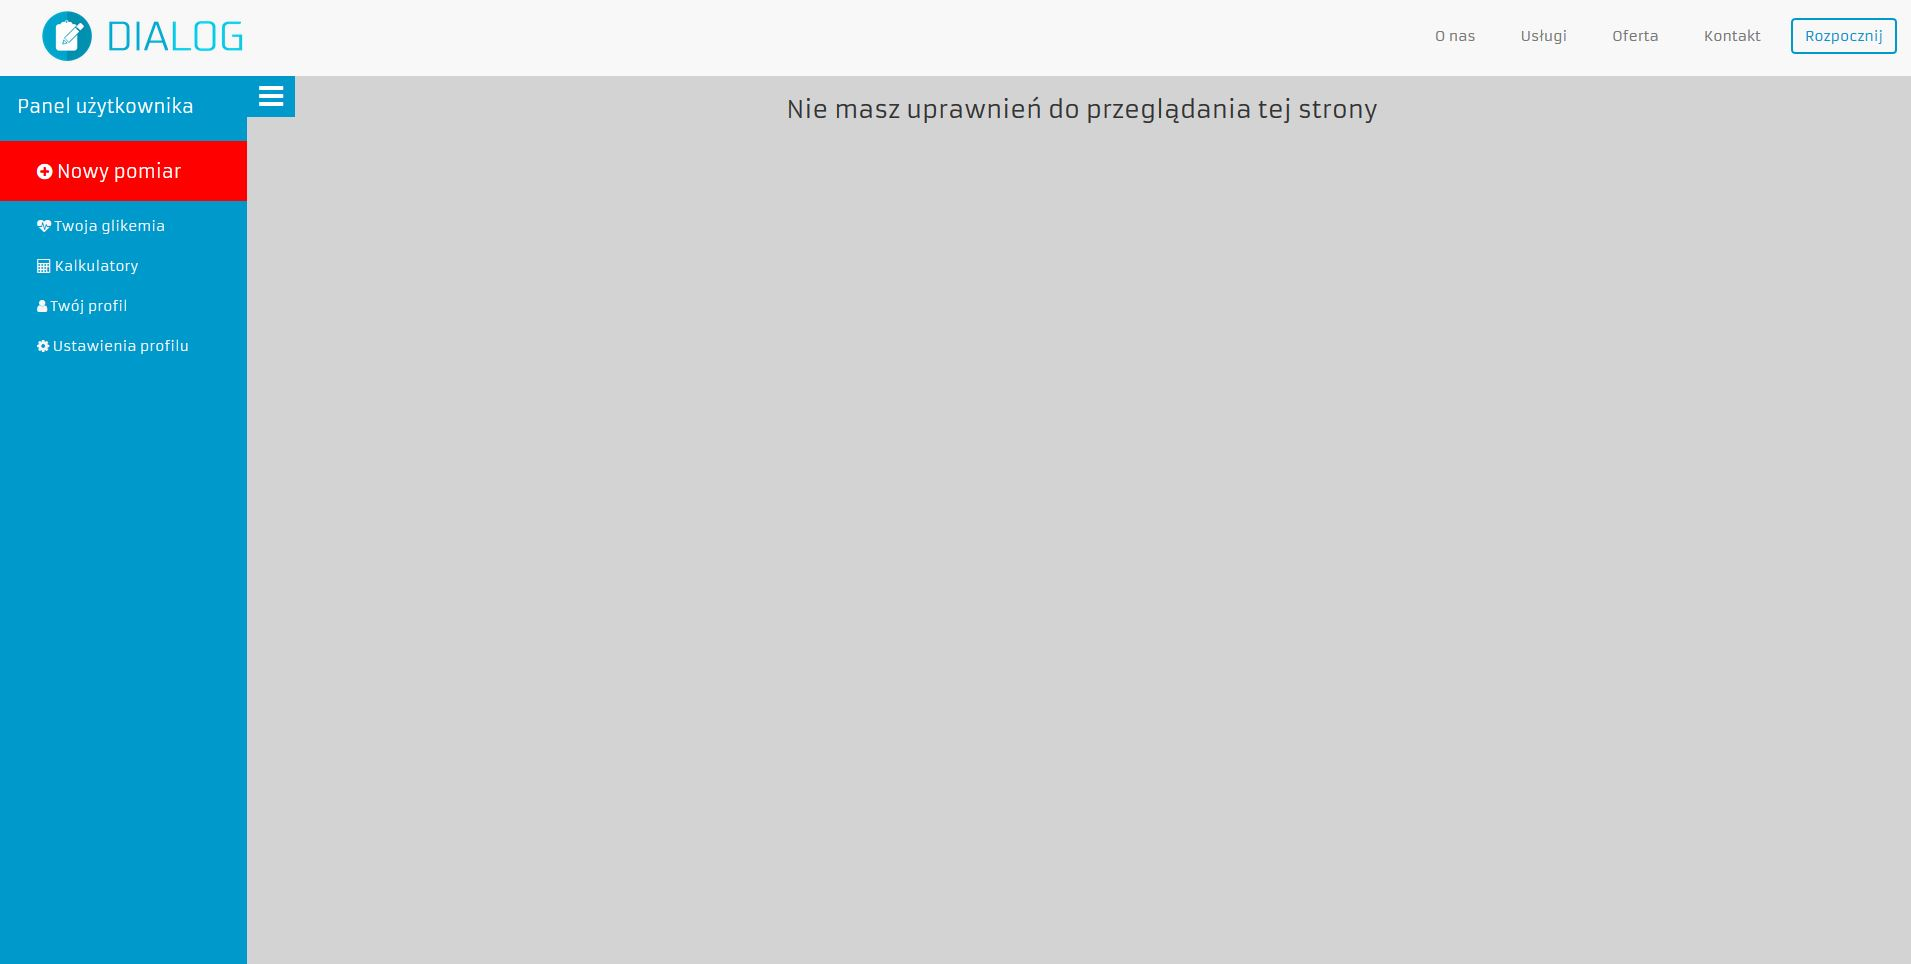
\includegraphics[scale=0.3]{images/no_access.jpg}
	\caption{Błąd przy próbie uzyskania dostępu do panelu użytkownika zalogowanego poprzez link URL}
	\label{Rys:no_access}
\end{figure}

Jak widać u góry (w menu górnym) nie ma dostępu do zakładki \textit{Twój dialog}, co oznacza, że użytkownik jest niezalogowany i próbuje uzyskać dostęp do linku URL udostępnianego wyłącznie użytkownikowi zalogowanemu. 

Podobna sytuacja tyczy się panelu administratora. Użytkownik nie posiadający w serwisie \textit{Auth0} roli \textit{Admin} nie posiada dostępu do funkcjonalności dla niej przeznaczonych. To oznacza, że nie da się uzyskać bezpośredniego dostępu do podstrony panelu administratora poprzez wklejenie linku URL do okna wyszukiwarki. Użytkownik przy takiej próbie zostaje natychmiastowo informowany właściwym komunikatem (rys. \ref{Rys:no_admin_access}).

\begin{figure}[h]
	\centering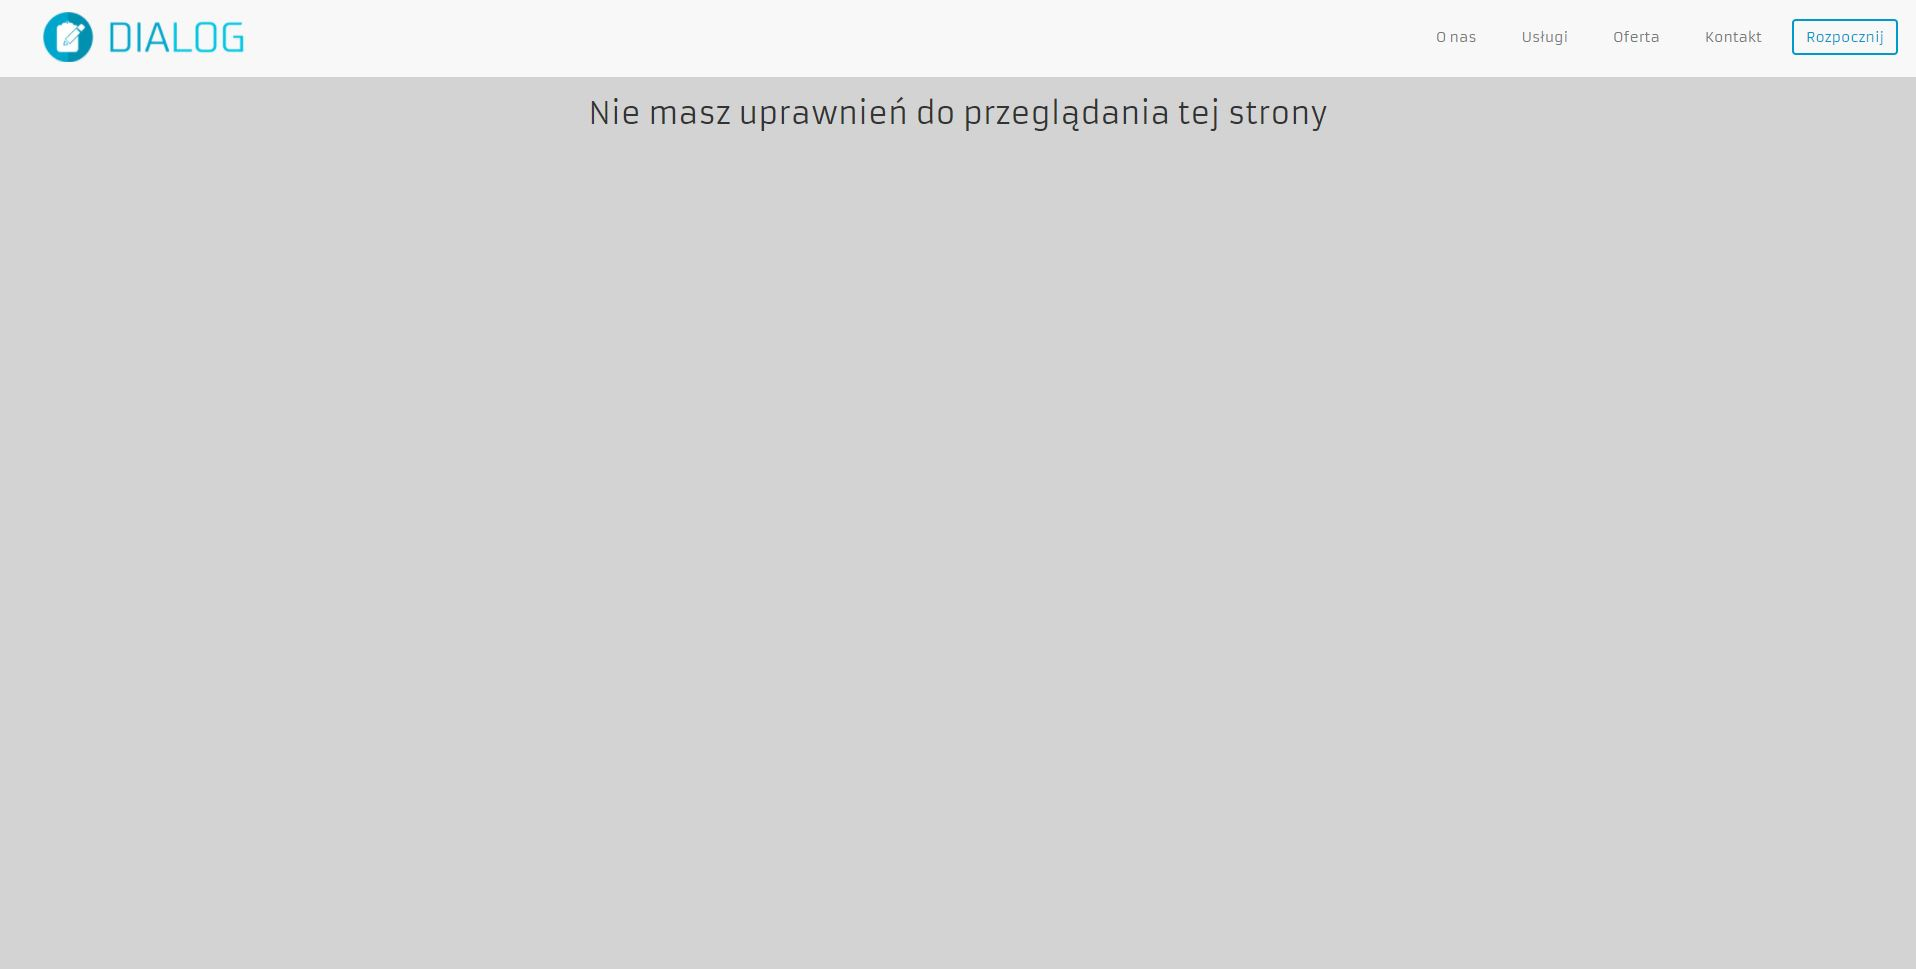
\includegraphics[scale=0.3]{images/no_admin_access.jpg}
	\caption{Błąd przy próbie uzyskania dostępu do panelu administratora poprzez link URL}
	\label{Rys:no_admin_access}
\end{figure}